\subsection{Proposed Pointing Strategies}
\label{sec:proposed_pointings}

For simplicity we chose to study one-year plans for an Extended
Mission, i.e., plans for Year 3 of the \tess mission. (Later in this
report we remark on some possible implications of our study for
additional years of an Extended Mission.)  Given the constraints
outlined in Sec.~\ref{sec:constraints_on_pointings}, we selected the
following scenarios for detailed study:

\begin{figure*}[!bt]
	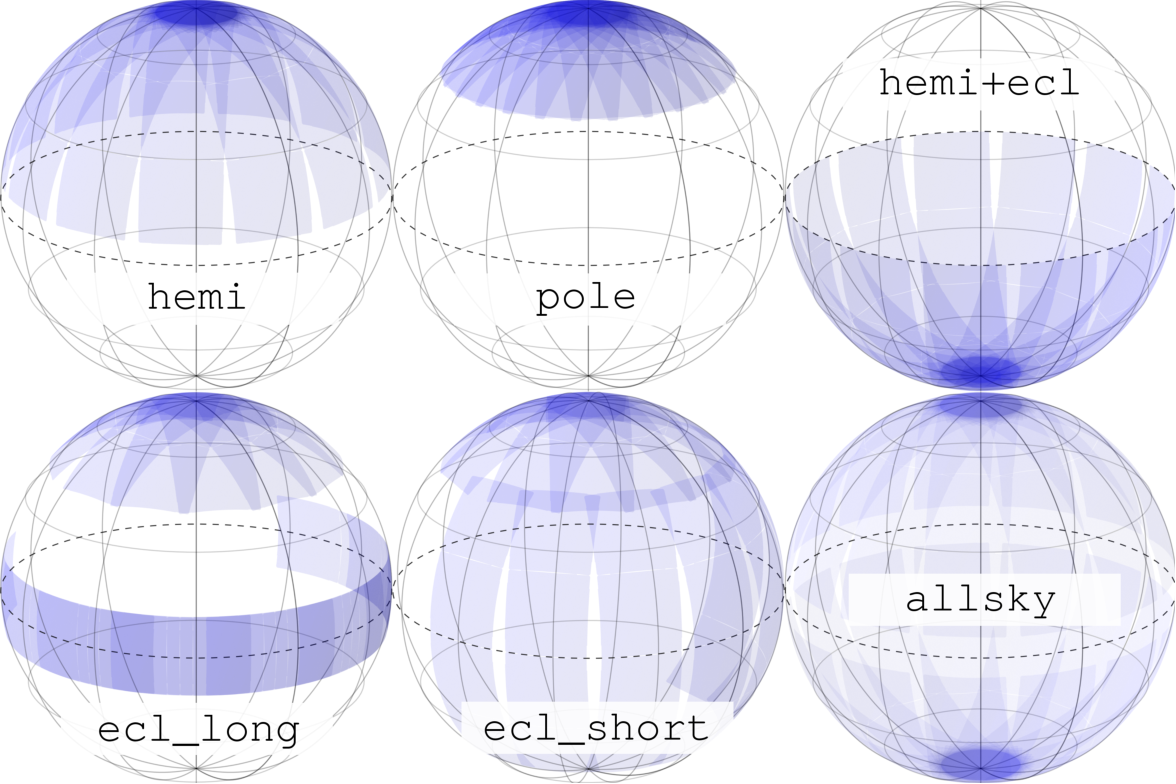
\includegraphics{figures/proposed_pointings_flat.pdf}
	\caption{Proposed pointing strategies for a \tess Extended Mission, visualized in ecliptic coordinates. \nhemi, \npole, \shemiAvoid, \elong, \eshort, and \hemis. Note for \elong\:and \eshort\:that Earth and moon crossings likely make an entire year looking at the ecliptic impractical (see Fig.~\protect\ref{fig:earth_moon_elong}).}
	\label{fig:proposed_pointings}
\end{figure*}

\begin{description}

\item[Scenario 1.] \nhemi: Repeat observations of one of the two
  ecliptic hemispheres in a manner similar to the Primary Mission.
  For concreteness we arbitrarily chose the northern ecliptic hemisphere
  for the third year. In this scenario we could take the opportunity to 
  shift the longitudes of all sectors by an amount that would enable 
  \tess to cover the gaps that were left during the Primary Mission 
  (the ``slits'' in the sky coverage between ecliptic latitudes of 
  6--30$^\circ$).
  However for simplicity, we opted to observe the same longitudes as
  in the Primary Mission.
  \textit{Motivation:} similar to the Primary Mission.
  Long time baseline at the North Ecliptic Pole, and broad sky
  coverage. Also remeasures transit times (and substantially improves 
  ephemerides)
  of previously detected \tess planets over most of the entire
  hemisphere.

\item[Scenario 2.] \npole: Focus on one of the ecliptic poles,
	arbitrarily chosen to be the north ecliptic pole for
	concreteness. \tesss sunshade and lens hoods must still
	suppress incoming sunlight in this scenario.
	A potential problem is sunlight might
	reflect off the interior of the sunshade and into a lens hood.
	Since this problem could be addressed by rotating the spacecraft to point slightly anti-Sun (putting the cameras in the shadow of the sunshade), we neglect any effects of extra
	 scattered sunlight ignored\footnote{whether this minor 
	adjustment would even be necessary depends on the combined performance of the
		sunshade and each camera's lens hood.
		These will be verified by measurements during commissioning.
		{\bf JNW: I don't understand the following sentence.} Note that the effect of the scattered sunlight is 
		maximal when the spacecraft is 
		at its furthest separation from the ecliptic plane, scaling with the 
		spacecraft's orbital inclination.}.
	\textit{Motivation:} maximizes the average duration of
	observations per star; intuitively expected to provide
	greatest sensitivity to long-period planets.

\item[Scenario 3.] \shemiAvoid: Repeat observations of one of the two
  ecliptic hemispheres, but in this case shifting all fields $6^\circ$
  toward the ecliptic, such that the combined fields-of-view reach all
  the way from the ecliptic to $6^\circ$ behind the ecliptic pole. We chose
  to simulate the southern ecliptic hemisphere because the northern
  version of this plan would suffer more from Earth and Moon interference
  (cf. Table~\ref{tab:dropped_fields} in
  Sec.~\ref{sec:earth_moon_crossings}).
  \textit{Motivation:} trades the long continuous viewing zone near
  the pole for greater sky coverage, and in particular, coverage of
  the ecliptic zone which was missed in the Primary Mission. Extensible
  to Year 4. Freshens ephemerides.
  
\item[Scenario 4.] \elong: Survey the ecliptic with 7 sectors (14
  orbits) in which the long axis of the fields-of-view are oriented
  along the ecliptic.  For the other 6 sectors, during the interval
  when ecliptic observations would be interrupted by Earth and Moon
  crossings, we focus on one of the ecliptic poles.
  \textit{Motivation:} covers the ecliptic, which will not be observed
  during the Primary Mission.  Offers opportunities for follow-up
  of K2 discoveries. Minimizes Earth-moon interference.
  
\item[Scenario 5.] \eshort: Survey the ecliptic and also cover a large
  fraction of the rest of the ecliptic hemisphere. For 7 sectors we
  observe the ecliptic but with the {\it short} axis oriented along
  the ecliptic, and the long axis reaching up to higher latitudes.
  The remaining 6 sectors are focused on the ecliptic pole, as in
  \elong.  \textit{Motivation:} similar to \elong, but with more
  overlap between this year and the Primary Mission to allow for
  improved transit ephemerides and better ability to follow-up on
  previous discoveries.
  Also covers more sky than \elong, which could improve the quantity
  of planet detections from full frame images.
  
\item[Scenario 6.] \hemis: Cover both northern and southern ecliptic
  hemispheres in a single year, by alternating between the hemispheres
  every 13.7 days.  \textit{Motivation:} rapid coverage of the
  entire sky, allows follow-up of almost all previously detected \tess
  objects and refined ephemerides.

\end{description}

Although these 6 scenarios seemed like reasonable choices for further study and direct
comparison, there are many other possibilities that may be of interest
that were not studied in detail, in order to keep the scope of this
report manageable.  Among these other possibilities that were considered but not studied are
\begin{itemize}
	\item The \npole\:strategy applied to the south ecliptic pole rather than the north (we do not expect major differences).
	\item The \nhemi\:strategy applied to the southern ecliptic hemipshere rather than the northern (we do not expect major differences).
	\item The \nhemi\:strategy, but rotated about the ecliptic polar axis by
	$12^\circ$ in longitude.
	\item The Northern inversion of \shemiAvoid, which is more strongly 
	affected by Earth and Moon crossings (Sec.~\ref{sec:earth_moon_crossings}) 
	and is less able to 
	improve knowledge of mid-transit times 
	(Fig.~\ref{fig:lowering_uncertainty_tc}).
	\item A version of \nhemi\ in which all fields are $12^\circ$ closer to 
    the ecliptic, rather than $6^\circ$ as in \shemiAvoid.
	\item A full year spent observing the ecliptic.  Such a plan would 
	suffer from Earth and Moon crossings for a substantial fraction of the year.
	We show the outage as a function of time in Fig.~\ref{fig:earth_moon_elong}.
	Solar system objects (planets, asteroids) could also be an annoyance, although
	we did not model their effects.
        \item Alternate between northern and southern ecliptic poles every 13.7 days.
        This would be similar to \hemis\:but would focus on the poles rather than the entire sky.
        It would sacrifice sky coverage (and ability to refresh ephemerides over the whole sky) in return for a longer mean  observation duration per star.
        \item Hybrid strategies that change from month to month.  For instance, in the \nhemi\:scenario, during a month when the Earth or Moon crosses through the field of a camera pointed close to the ecliptic, we could tilt all the cameras away from the ecliptic as in the \npole\:scenario.        
\end{itemize}
